%! Author = jonathan
%! Date = 5/26/25
\chapter{Related Work}\label{ch:related-work}
\noindent\textbf{Computation-Communication Overlap.}
To reduce the communication overheads of synchronization in distributed DNN training, many research efforts have been focused on
increasing the overlap of computation and communication.
For generic Transformer-based models without MoE layers,
many works~\cite{coconet,decomposition,centauri,t3,megascale,co2,syndicate,ccfuser,fused}
have provided insights and techniques to
partition and schedule computation and communication operations, a
imed at finer-grained overlapping.
To address the challenges posed by \alltoall communication and
expert parallelism in MoE training, Tutel~\cite{tutel} and FasterMoE~\cite{fastermoe}
overlap \alltoall with expert computation.
Lancet~\cite{lancet} additionally enables both non-MoE computation in
forward pass and weight gradient computation in backward pass to be overlapped with \alltoall.
Despite overlapping, the performance of these approaches is
limited in practice due to blocking synchronous collective communication with barriers.
In contrast, \sysname fundamentally
eliminates the inefficiencies with
asynchronous, device-initiated data transfers overlapped with tiled computation
all \emph{within a single kernel},
further differentiating itself from SOTA works~\cite{triton-dist, comet, deepep}
who also use this form of kernel-initiated communication but at a coarse-grained granularity
and without complete kernel fusion.
\chapter{Motivation}\label{ch:motivation}
\section{Straggler Effect}\label{subsec:straggler-effect}
\begin{figure}[!ht]
    \centering
     \begin{subfigure}{0.49\textwidth}
        \centering
        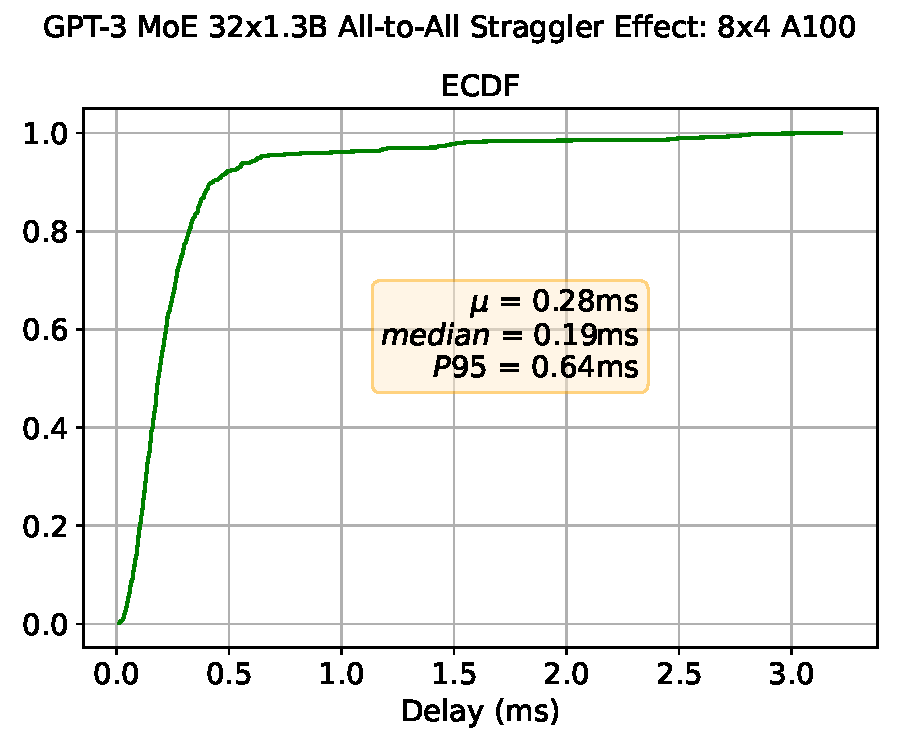
\includegraphics[width=\linewidth, keepaspectratio]{figures/GPT-3_MoE_32x1.3B_ecdf}
        \caption{ECDF}
        \label{sub:ecdf_perl}
    \end{subfigure}
    \begin{subfigure}{0.49\textwidth}
        \centering
        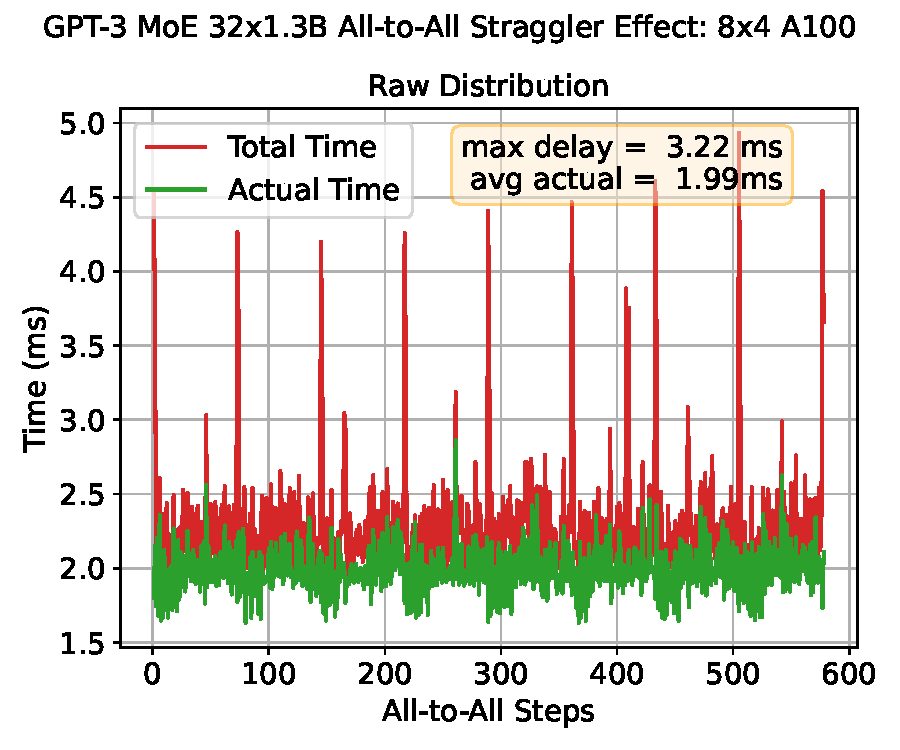
\includegraphics[width=\linewidth, keepaspectratio]{figures/GPT-3_MoE_32x1.3B}
        \caption{Raw Distribution}
        \label{sub:raw_perl}
    \end{subfigure}
    \vspace{1em} % space between rows
    \begin{subfigure}{0.49\textwidth}
        \centering
        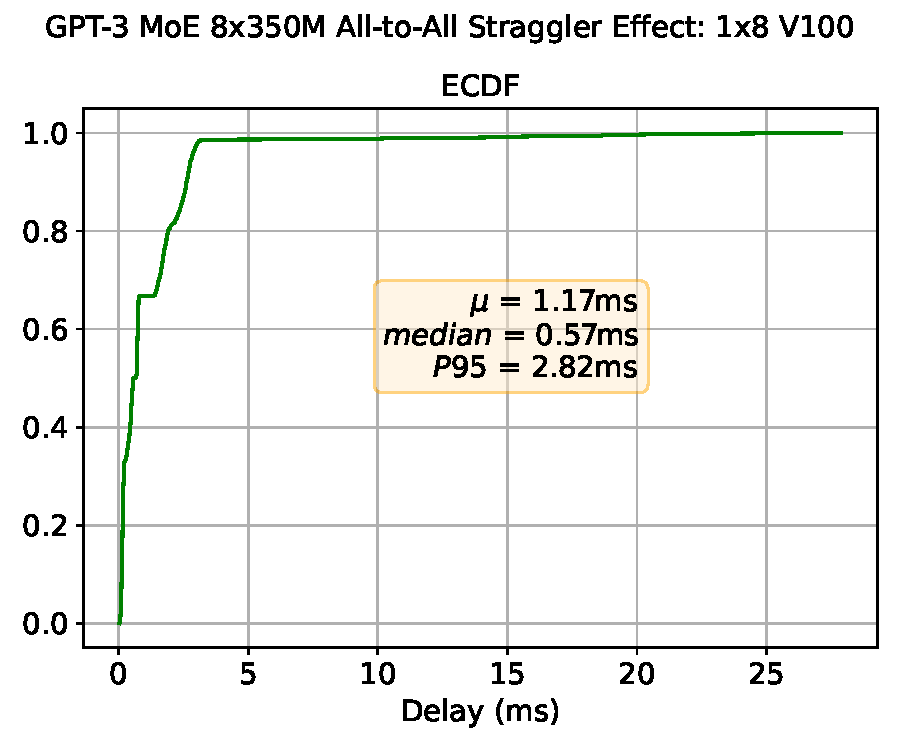
\includegraphics[width=\linewidth, keepaspectratio]{figures/GPT-3_MoE_8x350M_ecdf}
        \caption{ECDF}
        \label{sub:ecdf_az}
    \end{subfigure}
    \begin{subfigure}{0.49\textwidth}
        \centering
        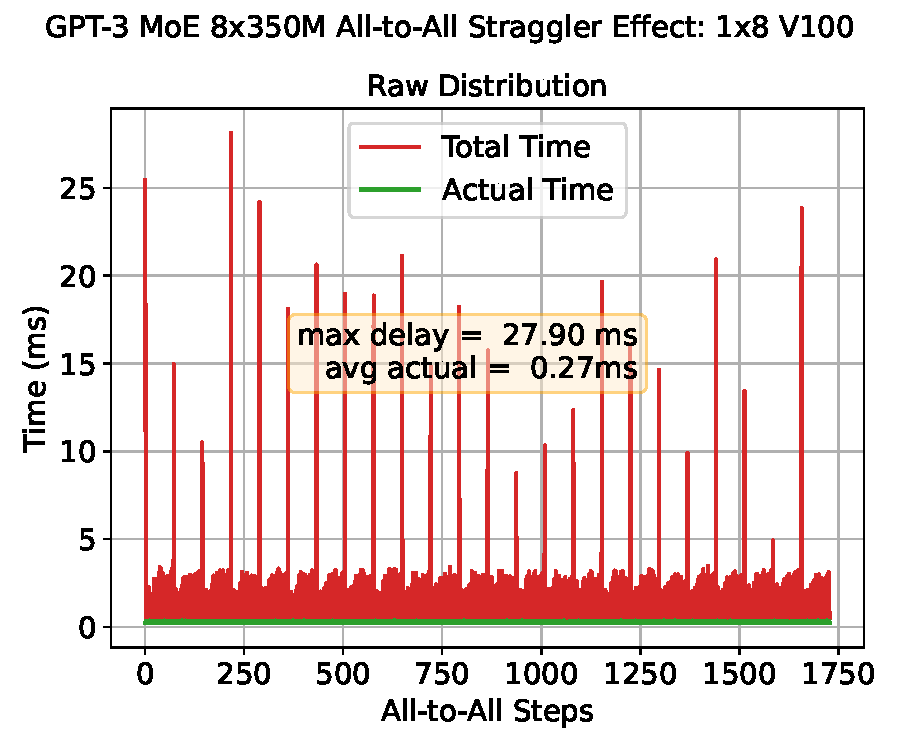
\includegraphics[width=\linewidth, keepaspectratio]{figures/GPT-3_MoE_8x350M}
        \caption{Raw Distribution}
        \label{sub:raw_az}
    \end{subfigure}
    \caption{Straggler effect of synchronous \alltoall. $M\times N$ A100 or V100 denotes
        $N$ GPUs within a node across $M$ nodes.
        Every GPU communicates with every other GPU per~\alltoall step.
        We capture the distribution of delay induced by stragglers across many steps.
        \textbf{Actual Time} $t_a$ denotes the fastest kernel execution time across all GPUs,
        conversely \textbf{Total Time} $t$ is the maximum recorded step time, while
        $Delay$ is the maximum difference between $t$ and $t_a$.}
    \label{fig:straggler}
\end{figure}
\begin{figure}[!ht]
    \centering
    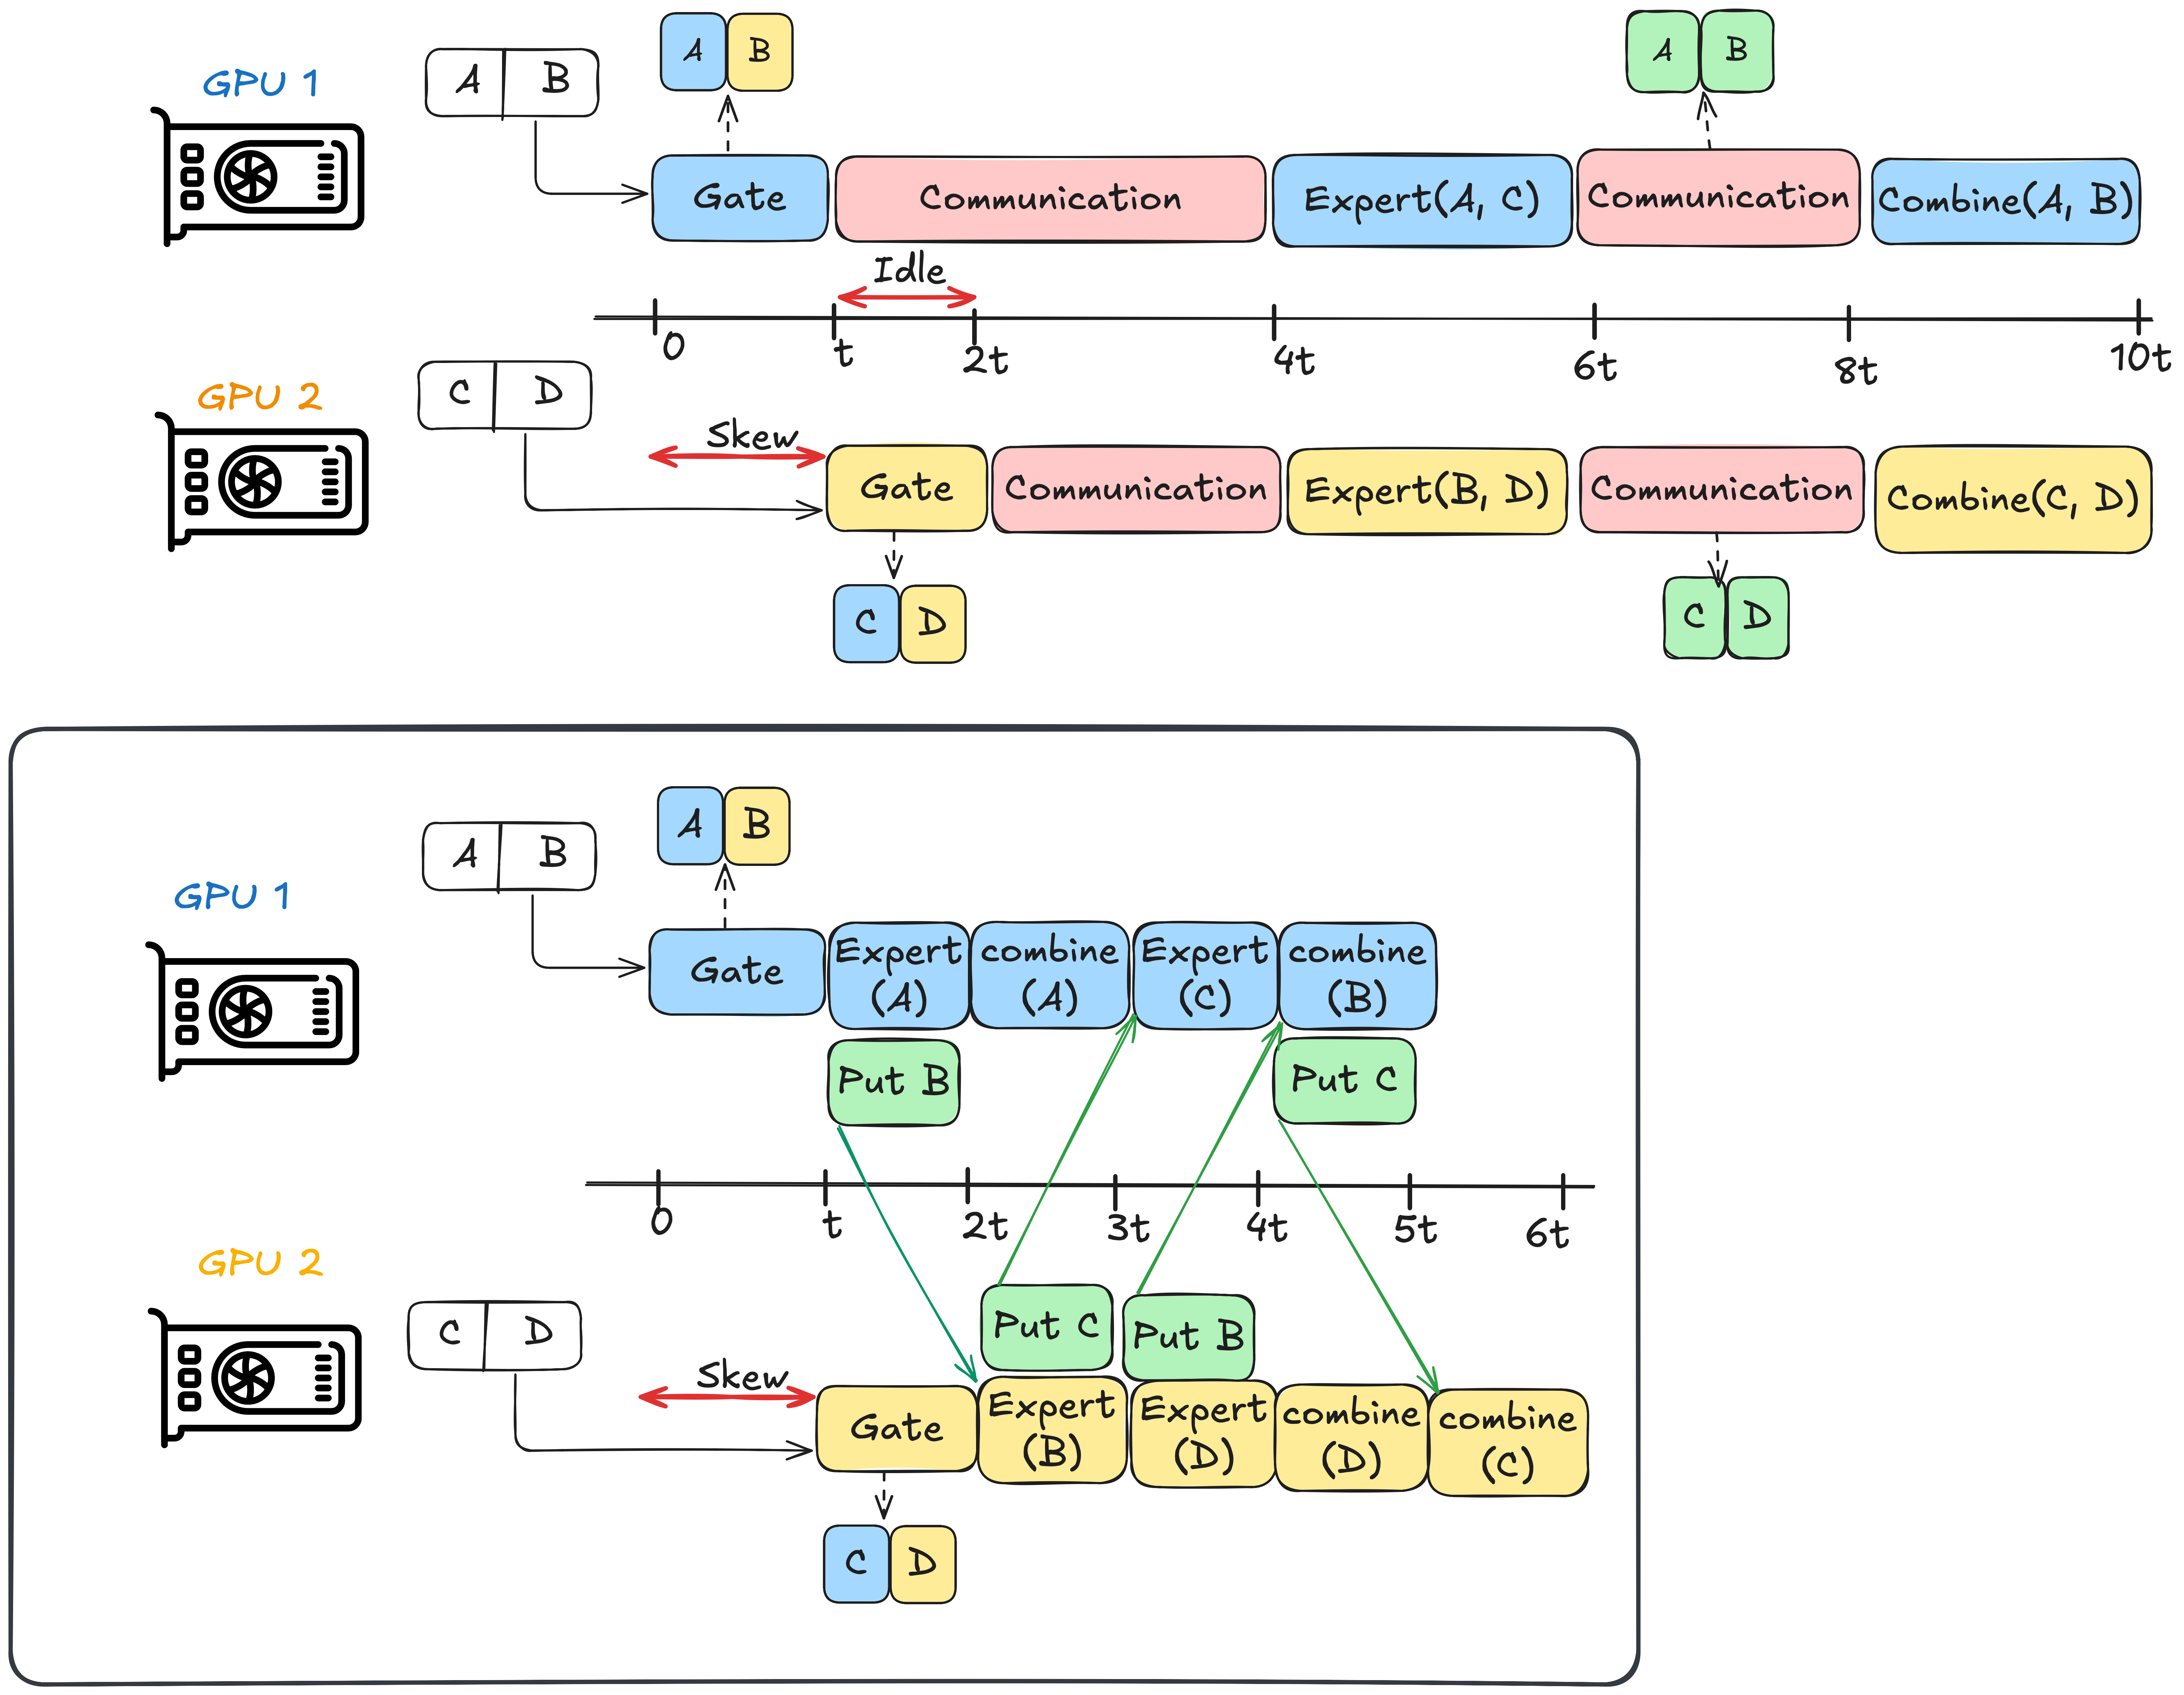
\includegraphics[width=0.98\textwidth, keepaspectratio]{figures/s_overlap}
    \caption{Overlapped Schedule (bottom) showing how idle time from the sequential schedule (top)
        is repurposed for computation. \sysname implements the overlapped schedule.}
    \label{fig:overlap}
\end{figure}
\alltoall communication as currently used in MoE frameworks is a ~\emph{synchronous} collective operation among
all participating GPUs. In this setting, disparities in processing speeds or kernel scheduling
among workers induce a straggler effect detrimental to the collective operation's performance.
Specifically, as shown in Figure~\ref{fig:straggler}, for distributed training of a 1.3B MoE model across 32 A100 GPUs,
we see P95 communication performance degradation of \textbf{1.32X} when compared to the mean actual kernel time
from Figure~\ref{sub:raw_perl}.
This performance reduction is rather tame as the underlying hardware is a supercomputer that is
well-tuned against ``software jitter''~\cite{nerscNetworkNERSC}.
On the other hand, the performance loss is more severe in a single node commodity Virtual Machine (VM) of
8 V100 GPUs with higher bandwidth, where we observe p95 performance reduction of \textbf{11X}.
In line with prior work~\cite{1639320, 10.1145/3545008.3545056} from the HPC community,
we argue that obviating the inherent barrier in this synchronous collective communication would
allow GPUs to repurpose this observed idle time for useful computation.
\section{Kernel Launch Overheads}\label{sec:kernel-launch-overheads}
\begin{figure}[!ht]
    \centering
    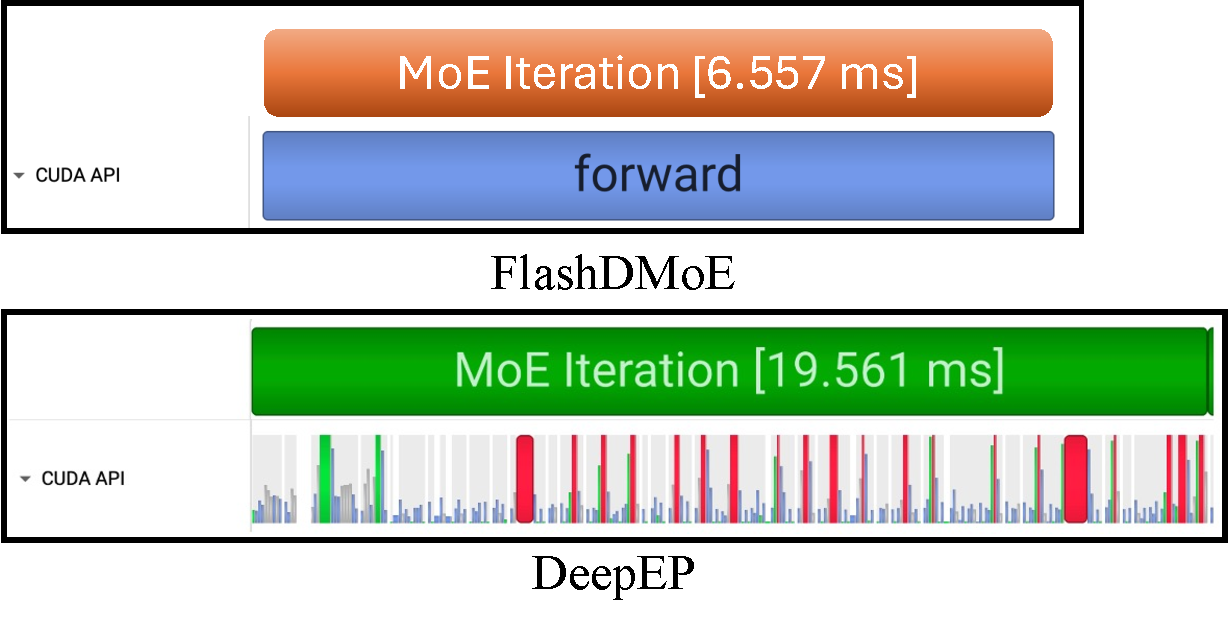
\includegraphics[width=0.8\textwidth, keepaspectratio]{figures/kernel_launch}
    \caption{Kernel Launch overhead (CUDA API row) juxtaposed with runtime latency.
    Compared to DeepEP that launches 432 kernels, \sysname launches a single one.}
    \label{fig:kl}
\end{figure}
We compare the kernel launch overheads between \sysname and existing baselines.
Table~\ref{tab:gpuOps} shows the number of kernel launches during a single forward pass: 
\sysname launches exactly one persistent kernel, 
while the baselines require up to 550 short-lived kernels.
Figure~\ref{fig:kl} visually compares \sysname and DeepEP~\cite{deepep} using CUDA API
traces captured by NSight Systems.
DeepEP exhibits numerous small CUDA API calls, while \sysname maintains high GPU
utilization by avoiding launch overhead and
synchronization gaps—achieving 93.17\% GPU utilization (\S\ref{ch:evaluation}) compared to 20.61\% for DeepEP.